\documentclass[12pt,a4paper]{article}

% ------------------------------------------------
% Pacotes
% ------------------------------------------------
\usepackage[utf8]{inputenc}
\usepackage[T1]{fontenc}
\usepackage[brazil]{babel}
\usepackage{graphicx}
\usepackage[table]{xcolor}
\usepackage{array}
\usepackage{tabularx}
\usepackage{geometry} 
\usepackage{float} 
\usepackage{fancyhdr}
\usepackage{mathptmx} % Times New Roman
\usepackage{enumitem}
\usepackage{amsfonts}
\usepackage{amsmath} % Recomendado para o comando \text{}
\usepackage{amssymb}
\usepackage{tikz}
\usetikzlibrary{positioning, shapes.geometric}
\usepackage{listings}
\usepackage{hyperref}
\lstset{
    language=Java,
    basicstyle=\small\ttfamily,
    keywordstyle=\bfseries,
    showstringspaces=false,
    breaklines=true,
    frame=none,
    numbers=none,
    tabsize=2,
    commentstyle=\itshape\color{gray},
    morekeywords={this}
}

% TikZ Styles for ER Diagrams
\tikzset{
    block/.style={rectangle, draw, thick, minimum width=2cm, minimum height=1cm, fill=white},
    diamond_node/.style={diamond, draw, thick, minimum width=2cm, minimum height=1cm, fill=white, aspect=2},
    attribute/.style={ellipse, draw, thin, minimum width=1.5cm, minimum height=0.6cm, fill=white, font=\scriptsize},
    line/.style={draw, thick}, 
}
% ------------------------------------------------ 
% Configuração de página
% ------------------------------------------------
\geometry{
    a4paper,
    left=2cm,
    right=2cm,
    top=2cm,
    bottom=2cm,
    headheight=15pt % Adicione isso
}
% Caixa para resposta discursiva
\newcommand{\resposta}[1]{
\noindent
\framebox[\textwidth]{
\begin{minipage}{0.98\textwidth}
\vspace{#1}
\end{minipage}
}
}

\pagestyle{fancy}
\fancyhf{}
\renewcommand{\headrulewidth}{0pt}

\setlength{\parindent}{0pt}

% ------------------------------------------------
% Comandos auxiliares
% ------------------------------------------------
\newcolumntype{L}[1]{>{\raggedright\arraybackslash}p{#1}}
\newcolumntype{C}[1]{>{\centering\arraybackslash}p{#1}}

% ------------------------------------------------
% Documento
% ------------------------------------------------
\begin{document}

% ------------------------------------------------
% Cabeçalho
% ------------------------------------------------
\begin{tabularx}{\textwidth}{@{} L{4cm} X @{}}
    \raisebox{-0.5cm}{
\includegraphics[width=4cm]{Universidade_de_Rio_Verde.jpg}} &
    \hfill
    \begin{tabular}{|>{\centering\arraybackslash}m{10cm}|>{\raggedright\arraybackslash}p{1.8cm}|}
        \hline
        \cellcolor{black}\color{white}\rule{0pt}{1.2cm}\textbf{LISTA DE EXERCÍCIOS} 
        & 
        \scriptsize Nota \tabularnewline
        \hline
    \end{tabular} 
\end{tabularx}
\vspace{0.3cm}

% ------------------------------------------------  
% Tabela principal
% ------------------------------------------------
\begin{tabularx}{\textwidth}{|X|L{2cm}|}
\hline
\textbf{Curso} & \textbf{Campus} \\
\textit{Engenharia de Software} & \textit{Rio Verde} \\
\hline
\multicolumn{2}{|l|}{ \textit{Programação Orientada a Objetos}} \\
\hline
\textbf{Nome do(a) acadêmico(a)} & \textbf{Valor} \\
 & 10,0 \\
\hline
\textbf{Professor} & \textbf{Turma} \\
\textit{ Sergio Souza Novak} & \textit{B} \\
\hline
\textbf{Data da Atividade} & \textbf{Código} \\
\textit{  /  /2026} & \textit{ESW448} \\
\hline
\end{tabularx}
 
% ------------------------------------------------
% Barra de Atenção
% ------------------------------------------------
\vspace{0.2cm}

\begin{tabularx}{\textwidth}{|X|}
\hline
\cellcolor{black}\color{white}
\centering \textbf{ATENÇÃO:} Esta atividade tem como objetivo a fixação e revisão dos conceitos de OO. \tabularnewline
\hline
\end{tabularx}

\vspace{0.3cm}

\textbf{ORIENTAÇÕES PARA A RESOLUÇÃO}  

\begin{itemize}
    \item Responda às questões com clareza;
    \item Desenvolva a interpretação crítica do código em Java;
\end{itemize}

\vspace{0.5cm}

\begin{center}
    \rule{\textwidth}{0.4pt}
    \textbf{QUESTÕES}
\end{center}

\vspace{0.5cm} 

\begin{enumerate}

    \item \textbf{Conceitos Fundamentais:} A partir dos textos de apoio abaixo:\\
    Um paradigma de programação pode ser entendido como um \textit{modelo} ou estilo que orienta a forma como programas de computador são concebidos e escritos. Em outras palavras, trata-se de um conjunto de conceitos, regras e práticas que guia o programador na maneira de estruturar o código, descrever as soluções e organizar os dados e as operações em um software. Paradigmas diferentes, como o imperativo, o funcional ou o orientado a objetos, oferecem visões distintas sobre como representar e resolver problemas por meio de algoritmos e linguagens de programação.

\noindent \textbf{Fonte:} \textit{Wikipédia. Paradigma de programação (pt.wikipedia.org/wiki/Paradigma\_de\_programação).}
    
    \begin{center}
        \includegraphics[width=0.8\textwidth]{tirinha1.png}
    \end{center}
    
    Com base nos seus conhecimentos sobre Programação Orientada a Objetos, explique com suas palavras o que é o paradigma de Orientação a Objetos e o que significa o conceito de Encapsulamento.
    
    \resposta{10cm}
    
    \vspace{0.3cm}

    \item \textbf{Construtores:} Qual é o principal objetivo da utilização de um método construtor em uma classe na Programação Orientada a Objetos?
    \begin{enumerate}[label=\Alph*)]
        \item Destruir o objeto da memória quando ele não é mais utilizado pelo sistema.
        \item Transformar a instância do objeto em uma representação textual.
        \item Inicializar os atributos do objeto com valores consistentes no momento de sua instanciação.
        \item Proteger os atributos de serem acessados por outras classes do sistema.
        \item Permitir que a classe seja herdada por múltiplas subclasses.
    \end{enumerate}

    \vspace{0.3cm}

    \item \textbf{Encapsulamento e Prática:} Observe o diagrama da classe \textbf{Produto} abaixo. Escreva o código Java para implementar esta classe, garantindo que o atributo \textbf{preco} seja inacessível diretamente de fora da classe (privado) e que existam métodos para obter o preço e aplicar um desconto. Desenvolva também um construtor apropriado.

    \begin{center} 
    \begin{tikzpicture}[node distance=0cm, outer sep=0pt, every node/.style={draw, rectangle, minimum height=0.6cm, font=\small\ttfamily, anchor=north west}]
        \node (header) [fill=white, minimum width=9cm, font=\small\bfseries] at (0,0) {Produto};
        
        \node (attrs) [minimum width=9cm, align=left] at (0,-0.6cm) {
            - nome : String \\
            - preco : double \\
            + Produto(nome: String, preco: double) \\
            + getPreco() : double \\
            + aplicarDesconto(percentual: double) : void
        };
    \end{tikzpicture}
    \end{center}

    \resposta{15cm}

    \vspace{0.3cm}

    \item Em programação orientada a objetos, métodos de acesso do tipo \textit{getter} (métodos de consulta) têm como principal responsabilidade:
    \begin{enumerate}[label=\Alph*)]
        \item retornar o valor atualmente armazenado em um atributo encapsulado.
        \item alterar o estado interno de um objeto por meio de regras de negócio.
        \item garantir que o objeto instanciado seja deletado da memória.
        \item conectar a instância do objeto a uma base de dados relacional.
        \item construir uma nova instância da classe em memória, semelhante ao construtor.
    \end{enumerate}

    \vspace{0.3cm}

    \item  O encapsulamento em Orientação a Objetos é um dos pilares fundamentais. Sobre os modificadores de visibilidade (público, privado, protegido) na maioria das linguagens OO, indique a alternativa \textbf{correta}:
    \begin{enumerate}[label=\Alph*)]
        \item Um atributo público só é acessível na classe onde foi declarado.
        \item Um método protegido é visível dentro da própria classe, nas suas subclasses e geralmente no mesmo pacote.
        \item Um atributo privado pode ser acessado diretamente pelas subclasses, visando facilitar a herança.
        \item Membros privados podem ser modificados deliberadamente por qualquer classe que instancie o objeto, desde que autorizados.
        \item Um método público não consegue acessar métodos ou atributos privados da sua própria classe em nenhuma hipótese.
    \end{enumerate} 

    \vspace{0.3cm}

    \item \textbf{Agricultura 4.0 — Estufa Inteligente:} A modelagem da classe \texttt{EstufaInteligente} controla variáveis ambientais para otimizar o plantio, em substituição direta a fornos industriais.

    \begin{center}
    \begin{tikzpicture}[node distance=0cm, outer sep=0pt, every node/.style={draw, rectangle, minimum height=0.6cm, font=\small\ttfamily, anchor=north west}]
        \node (header) [fill=white, minimum width=9cm, font=\small\bfseries] at (0,0) {EstufaInteligente};
        
        \node (attrs) [minimum width=9cm, align=left] at (0,-0.6cm) {
            - umidadeAtual : double \\
            - umidadeMinima : double \\
            - umidadeMaxima : double \\
            - sistemaAtivo : boolean \\
            - aguaConsumida : double \\
            + EstufaInteligente(uMin: double, uMax: double) \\
            + ligar() : void \\
            + desligar() : void \\
            + irrigar(litros: double) : double \\
            + colherFrutos() : double \\
            - umidadeIdeal() : boolean \\
            - verificarSeguranca() : void
        };
    \end{tikzpicture}
    \end{center}
\begin{small}
\begin{lstlisting}
01: // EstufaInteligente.java
02: public class EstufaInteligente {
03:     private double umidadeAtual;
04:     private double umidadeMinima;
05:     private double umidadeMaxima;
06:     private boolean sistemaAtivo;
07:     private double aguaConsumida;
08: 
09:     public EstufaInteligente(double uMin, double uMax) {
10:         this.umidadeMinima = uMin;
11:         this.umidadeMaxima = uMax;
12:         this.umidadeAtual = 40.0;
13:         this.sistemaAtivo = false;
14:     }
15: 
16:     public void ligar() { this.sistemaAtivo = true; }
17:     public void desligar() { this.sistemaAtivo = false; }
18: 
19:     public double irrigar(double litros) {
20:         this.umidadeAtual += litros * 5;
21:         this.aguaConsumida += litros;
22:         verificarSeguranca();
23:         return this.umidadeAtual;
24:     }
25: 
26:     public double colherFrutos() {
27:         if (sistemaAtivo && umidadeIdeal()) {
28:             return 50.0; // Producao em kg
29:         }
30:         return 0.0;
31:     }
32: 
33:     private boolean umidadeIdeal() {
34:         return umidadeAtual >= umidadeMinima && umidadeAtual <= umidadeMaxima;
35:     }
36: 
37:     private void verificarSeguranca() {
38:         if (umidadeAtual > umidadeMaxima) {
39:             desligar();
40:         }
41:     }
42: }
\end{lstlisting}
\end{small}

    Considerando o código da classe \texttt{EstufaInteligente}, julgue as afirmações como Verdadeiras (V) ou Falsas (F) e assinale a sequência \textbf{correta}:

    ( ) O método \texttt{umidadeIdeal} (linhas 33-35) é privado, o que significa que ele só pode ser invocado internamente pelos métodos da própria classe. \\
    ( ) Na chamada do método \texttt{irrigar}, a verificação de segurança é sempre ativada internamente e garante o desligamento automático do equipamento caso a umidade supere o limite máximo permitido. \\
    ( ) O processo de colher frutos (linha 26) acontece independentemente de o sistema da estufa estar ligado ou desligado. \\
    ( ) É plenamente possível que uma classe em outro pacote altere de forma direta e irrestrita o valor do atributo \texttt{aguaConsumida}.

    \begin{enumerate}[label=\Alph*)]
        \item V - V - F - F.
        \item V - F - V - V.
        \item F - V - V - F.
        \item V - V - V - F.
        \item F - F - F - V.
    \end{enumerate}


    \vspace{0.3cm}


    \item Assinale a alternativa que apresenta de forma correta o modificador de acesso (ou a falta dele) em Java que permite que um membro de uma classe seja acessado \textbf{apenas} por classes que pertençam ao mesmo pacote (modificador default):
    \begin{enumerate}[label=\Alph*)]
        \item \texttt{private}
        \item \texttt{protected}
        \item \textit{package-private} (omissão de modificador)
        \item \texttt{public}
        \item \texttt{static default}
    \end{enumerate}

    \vspace{0.3cm}

    \item \textbf{Modificador \texttt{protected}:} Considerando os conceitos de orientação a objetos em Java, assinale a alternativa que descreve com sucesso quem possui permissão padrão para acessar o atributo \texttt{codigoAcesso} declarado no código abaixo:

\begin{lstlisting}
package sistema.seguranca; 
public class Catraca {       
    protected int codigoAcesso; 
}
\end{lstlisting}

    \begin{enumerate}[label=\Alph*)]
        \item Somente classes filhas de \texttt{Catraca}, independentemente do pacote, sem acesso para outras classes do mesmo pacote.
        \item Classes que estejam no mesmo pacote (\texttt{sistema.seguranca}) de \texttt{Catraca} ou classes filhas (subclasses), mesmo que estejam em outros pacotes.
        \item Qualquer classe, em qualquer pacote, desde que devidamente instanciada na memória principal.
        \item Exclusivamente os métodos que pertencem internamente à declaração da classe \texttt{Catraca}.
        \item Apenas as classes filhas que estiverem rigorosamente contidas dentro do mesmo pacote (\texttt{sistema.seguranca}).
    \end{enumerate}

    \vspace{0.3cm}

\item Leia o texto de apoio e responda o que se pede:

Um \textit{ensemble}, no contexto de aprendizado de máquina e inteligência artificial, é uma técnica que combina múltiplos modelos preditivos (como redes neurais, árvores de decisão ou SVMs) com o objetivo de obter uma performance superior à de um único modelo individual. A ideia central é explorar a diversidade entre os modelos, pois cada um pode capturar aspectos diferentes dos dados. Dessa forma, é possível reduzir erros sistemáticos e aumentar a robustez geral das previsões por meio de métodos como votação majoritária (para tarefas de classificação) ou média ponderada (para problemas de regressão).

Entre as principais abordagens de \textit{ensemble learning} destacam-se três técnicas. A primeira é o \textit{bagging} (\textit{Bootstrap Aggregating}), utilizado por algoritmos como o \textit{Random Forest}, que consiste em treinar diversos modelos independentes utilizando subconjuntos aleatórios dos dados. A segunda é o \textit{boosting}, presente em algoritmos como \textit{AdaBoost} e \textit{XGBoost}, no qual os modelos são treinados de forma sequencial, dando maior atenção aos exemplos que foram classificados incorretamente pelos modelos anteriores. Por fim, há o \textit{stacking}, que utiliza um modelo adicional, chamado de meta-modelo, responsável por combinar as previsões produzidas pelos modelos base.

\noindent \textbf{Fonte:} \textit{Wikipédia. Ensemble learning}. Disponível em: \url{https://pt.wikipedia.org/wiki/Ensemble_learning}.

\vspace{0.4cm}



Com base nas informações do texto e nos seus conhecimentos sobre Programação Orientada a Objetos, analise o código Java abaixo que propõe uma modelagem simplificada de uma técnica de \textit{ensemble}:

\begin{lstlisting}
public class Ensemble {
    private String tipoAbordagem;
    private int quantidadeModelosBase;
    private double acuraciaGeral;

    public Ensemble(String tipo, int qtdeModelos) {
        this.tipoAbordagem = tipo;
        this.quantidadeModelosBase = qtdeModelos;
        this.acuraciaGeral = 0.0;
    }

    public void registrarAcuracia(double novaAcuracia) {
        if (novaAcuracia >= 0.0 && novaAcuracia <= 100.0) {
            this.acuraciaGeral = novaAcuracia;
        }
    }

    public double getAcuraciaGeral() {
        return this.acuraciaGeral;
    }
}
\end{lstlisting} 
\begin{figure}[h]
\centering
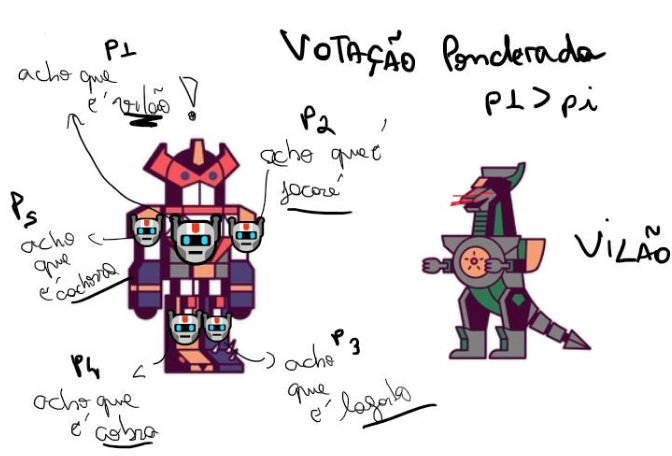
\includegraphics[width=0.7\textwidth]{ensemble.png}
\caption{Fonte: Cadernos de desenho do professor Sergio. O ensemble é como se fosse um megazord da Inteligência Artificial.} 
\end{figure}
 
Considerando as boas práticas arquiteturais e regras de visibilidade (encapsulamento), assinale a alternativa \textbf{correta}:
\begin{enumerate}[label=\Alph*)]
    \item Os atributos \texttt{tipoAbordagem} e \texttt{quantidadeModelosBase} deveriam ter a visibilidade \texttt{public} para facilitar suas alterações irrestritas durante a fase de acréscimo de novos sub-modelos.
    \item A alteração direta e externa do atributo usando \texttt{meuEnsemble.acuraciaGeral = -10.5;} é plenamente permitida, desde que a linguagem identifique que seja a classe principal do sistema.
    \item O método \texttt{registrarAcuracia()} permite a alteração de estado da variável sem aplicar nenhum filtro prático limitante de validade para o valor de \texttt{acuraciaGeral}. 
    \item O método construtor inicializa a variável \texttt{acuraciaGeral} com \texttt{0.0} toda vez que um novo objeto \texttt{Ensemble} é recém-instanciado na memória.
    \item Qualquer classe, em qualquer pacote, tem total acesso ao método \texttt{getAcuraciaGeral()}, porém é impedida de examinar o número devolvido visto que a variável que o preenche é declarada como \texttt{private}.
\end{enumerate}
    \item No contexto de IoT nas cidades e campos modernos, modelou-se uma classe representante de um VANT (Veículo Aéreo Não Tripulado).

    \begin{center}
    \begin{tikzpicture}[node distance=0cm, outer sep=0pt, every node/.style={draw, rectangle, minimum height=0.6cm, font=\small\ttfamily, anchor=north west}]
        \node (header) [fill=white, minimum width=9cm, font=\small\bfseries] at (0,0) {DronePulverizador};
        
        \node (attrs) [minimum width=9cm, align=left] at (0,-0.6cm) {
            - modelo : String \\
            - bateriaAtual : double \\
            - capacidadePesticida : double \\
            - nivelPesticida : double \\
            - emVoo : boolean \\
            + DronePulverizador(modelo: String, cap: double) \\
            + decolar() : void \\
            + pousar() : void \\
            + pulverizar(area: double) : boolean \\
            - consumirBateria(area: double) : void
        };
    \end{tikzpicture}
    \end{center}
\begin{small}
\begin{lstlisting}
01: public class DronePulverizador {
02:     private String modelo;
03:     private double bateriaAtual;
04:     private double capacidadePesticida;
05:     private double nivelPesticida;
06:     private boolean emVoo;
07: 
08:     public DronePulverizador(String mod, double cap) {
09:         this.modelo = mod;
10:         this.capacidadePesticida = cap;
11:         this.nivelPesticida = cap; // tanque abastecido
12:         this.bateriaAtual = 100.0;
13:         this.emVoo = false;
14:     }
15: 
16:     public void decolar() { 
17:         if(this.bateriaAtual > 20.0) { this.emVoo = true; }
18:     }
19:     public void pousar() { this.emVoo = false; }
20: 
21:     public boolean pulverizar(double area) {
22:         if (!this.emVoo) { return false; }
23:         double gasto = area * 0.5;
24:         if (this.nivelPesticida >= gasto) {
25:             this.nivelPesticida -= gasto;
26:             consumirBateria(area);
27:             return true;
28:         }
29:         return false;
30:     }
31: 
32:     private void consumirBateria(double area) {
33:         this.bateriaAtual -= area * 1.5;
34:         if (this.bateriaAtual <= 20.0) {
35:             this.pousar(); // pouso de emergencia provocado
36:         }
37:     }
38: }
\end{lstlisting}
\end{small}

    Com base no código da classe \texttt{DronePulverizador}, analise as afirmações abaixo e assinale a alternativa que apresenta a sequência \textbf{correta} respectiva (V para Verdadeiro e F para Falso):

    ( ) O método \texttt{consumirBateria} possui visibilidade privada (linha 32), impedindo sua chamada direta externa por outras classes e sendo o responsável, se necessário, por disparar um pouso forçado de emergência. \\
    ( ) O drone sempre decola (muda o estado \texttt{emVoo} para \texttt{true}) cada vez que o método \texttt{decolar} é chamado no sistema principal, não importando como está seu nível de bateria naquele momento. \\
    ( ) O drone em momento algum injeta defensivo se não estiver garantidamente em estado de voo ativo e não possuir pesticida em quantidade suficiente no seu tanque. \\
    ( ) A leitura direta da \texttt{bateriaAtual} bem como sua alteração arbitrária por qualquer classe em outro arquivo é aceitável, visto que o atributo é deixado visível.

    \begin{enumerate}[label=\Alph*)]
        \item V - F - V - F.
        \item F - V - F - V.
        \item V - V - F - F.
        \item F - F - V - V.
        \item V - F - F - V.
    \end{enumerate}

    \vspace{0.3cm}

    \item Considere a modelagem de uma classe \texttt{Termostato} (usada em aparelhos de Ar Condicionado Inteligentes) que possui um atributo restrito e fortemente encapsulado, denominado \texttt{temperaturaDesejada}.

    \begin{center}
    \begin{tikzpicture}[node distance=0cm, outer sep=0pt, every node/.style={draw, rectangle, minimum height=0.6cm, font=\small\ttfamily, anchor=north west}]
        \node (header) [fill=white, minimum width=9cm, font=\small\bfseries] at (0,0) {Termostato};
        
        \node (attrs) [minimum width=9cm, align=left] at (0,-0.6cm) {
            - temperaturaDesejada : double \\
            + getTemperatura() : double \\
            + setTemperatura(temp: double) : void
        };
    \end{tikzpicture}
    \end{center}

    Explique, conceitualmente, a extrema importância de se utilizar abordagens controladas via métodos \textit{getters} e \textit{setters} em vez de permitir o acesso e intervenção direta no atributo \texttt{temperaturaDesejada} (\textbf{limite-se apenas à linguagem humana verbal escrita, sem programação}). 
    Complementarmente, dê um bom exemplo lúdico de regra de negócio/controle de limites que faria todo sentido e poderia ser codificada no corpo do método \texttt{setTemperatura(temp: double)}, evitando falhas do dispositivo de refrigeração.

    \resposta{13cm}

    \vspace{0.3cm}
    
    \item Leia o texto e responda o que se pede: \\
    O carrinho de compras na internet é uma funcionalidade essencial dos sites de comércio eletrônico, responsável por reunir de forma organizada os itens selecionados pelo consumidor ao longo da navegação. Ele funciona como um espaço virtual onde os produtos escolhidos são armazenados temporariamente, permitindo adicionar, remover ou alterar quantidades antes da finalização do pedido, espelhando o comportamento do carrinho físico em uma loja tradicional.

\noindent \textbf{Fonte:} \textit{Shopify. Carrinho de compras online (www.shopify.com/br/blog/carrinho-de-compras-online).}
    
    
    
    Analise o trecho de código Java abaixo, que modela um \texttt{CarrinhoDeCompras}.

\begin{lstlisting}
public class CarrinhoDeCompras {
    private double totalCompras;

    public CarrinhoDeCompras() {
        this.totalCompras = 0.0;
    }

    public void adicionarItem(double preco) {
        if (preco > 0) {
            this.totalCompras += preco;
        }
    }
    
    // Metodo Y
}
\end{lstlisting}

    Qual das opções abaixo representa o código correto para o "\texttt{Metodo Y}", de forma a respeitar o encapsulamento, permitindo que o valor total seja lido, porém sem permitir que o valor do atributo \texttt{totalCompras} seja modificado diretamente de fora da classe?
    \begin{enumerate}[label=\Alph*)]
        \item \texttt{public void setTotalCompras(double total) \{ this.totalCompras = total; \}}
        \item \texttt{public double getTotalCompras() \{ return this.totalCompras; \}}
        \item \texttt{private double lerTotal() \{ return totalCompras; \}}
        \item \texttt{public double getAndSetTotal(double total) \{ this.totalCompras = total; return total; \}}
        \item \texttt{protected void exibirTotal() \{ System.out.println(totalCompras); \}}
    \end{enumerate}

    \vspace{0.3cm}
    
    \item Considere a classe \texttt{BateriaSmartphone} descrita a seguir e marque Verdadeiro (V) ou Falso (F) para as afirmações sobre a sua estrutura.

\begin{lstlisting}
public class BateriaSmartphone {
    private int carga;

    public BateriaSmartphone() {
        this.carga = 100;
    }

    public void usarBateria(int consumo) {
        if (this.carga - consumo >= 0) {
            this.carga -= consumo;
        } else {
            this.carga = 0;
        }
    }
    
    public void carregarBateria(int quantidade) {
        this.carga += quantidade;
        if (this.carga > 100) {
            this.carga = 100;
        }
    }
    
    public int getCarga() {
        return this.carga;
    }
}
\end{lstlisting}

    ( ) A classe não protege adequadamente o atributo \texttt{carga}, pois qualquer outra classe pode facilmente instanciar o objeto e usar \texttt{bateria.carga = 200;}. \\
    ( ) Os métodos \texttt{usarBateria} e \texttt{carregarBateria} garantem a integridade dos dados e impõem limites de regra de negócio, impedindo a carga de ficar negativa ou superior a 100. \\
    ( ) O método construtor garante que, toda vez que um novo objeto \texttt{BateriaSmartphone} for instanciado na memória, ele inicie sempre com sua carga em 100. \\
    ( ) O único método através do qual agentes externos a esta classe conseguem saber a quantidade exata de carga de energia restante é utilizando o \texttt{getCarga()}.
    
    \begin{enumerate}[label=\Alph*)]
        \item V - V - V - F.
        \item F - V - V - V.
        \item V - F - V - V.
        \item F - F - V - V.
        \item F - V - F - V.
    \end{enumerate}

    \vspace{0.3cm}

    \item \textbf{Prática de Código (Discursiva):} A classe abaixo representa um \texttt{Funcionario} com salário encapsulado. No entanto, ela necessita de um método que conceda um aumento ao funcionário com base em uma porcentagem (ex: 10\%).  

\begin{lstlisting}
public class Funcionario {
    private String nome;
    private double salario;

    public Funcionario(String nome, double salario) {
        this.nome = nome;
        this.salario = salario;
    }

    public double getSalario() {
        return this.salario;
    }
    
    // Escreva o metodo de aumento aqui
}
\end{lstlisting}

    Escreva, em sintaxe Java, o método \texttt{aplicarAumento(double porcentagem)} que deve ser inserido na classe. O método não deve retornar nada (\texttt{void}), mas deve alterar o valor do atributo \texttt{salario} somando o correspondente da porcentagem passada como parâmetro. Adicione também uma verificação simples: apenas conceda o aumento se a porcentagem for maior que zero.

    \resposta{8cm}



\vspace{0.8cm}


\item Leia o texto de apoio e responda o que se pede:

Um \textit{overfitting} ocorre quando um modelo de aprendizado de máquina aprende os dados de treinamento com excesso de detalhe, capturando não apenas os padrões gerais, mas também ruídos e peculiaridades específicas do conjunto de treino. Isso faz com que o modelo apresente excelente performance nos dados de treinamento, mas generalize mal para novos dados não vistos, resultando em alta variância e baixa capacidade de predição em situações reais.

Por outro lado, o \textit{underfitting} acontece quando o modelo é incapaz de capturar adequadamente os padrões subjacentes dos dados, apresentando performance ruim tanto no conjunto de treinamento quanto nos dados de teste. Esse problema está geralmente associado a modelos excessivamente simples ou com tempo de treinamento insuficiente, caracterizando-se por alta viés e incapacidade de aprender a complexidade inerente aos dados.

\noindent \textbf{Fonte:} \textit{Wikipédia. Overfitting e Underfitting}. Disponível em: \url{https://pt.wikipedia.org/wiki/Overfitting}.

\begin{figure}[H]
    \centering
    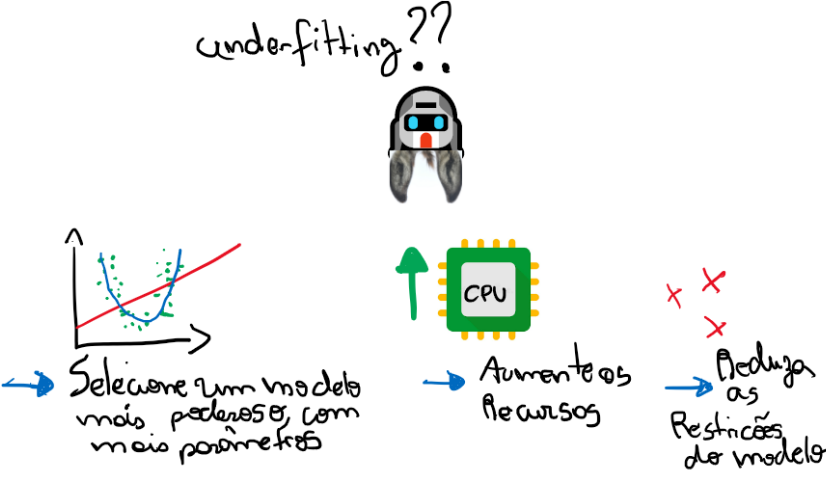
\includegraphics[width=0.7\textwidth]{underfitting.png}
    \caption{Ilustração de Underfitting.}
    \vspace{0.3cm}
    
    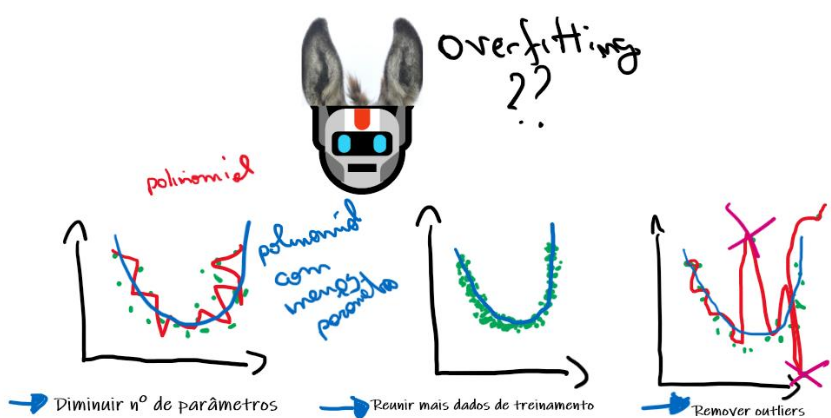
\includegraphics[width=0.7\textwidth]{overfitting.png}
    \caption{Ilustração de Overfitting.}
    
    \vspace{0.3cm}
    {\footnotesize Fonte: Cadernos de desenho do professor Sergio.}
\end{figure}

Com base nas ilustrações acima e nos conceitos de Programação Orientada a Objetos, analise a implementação da classe \texttt{ModeloIA} abaixo:

\begin{lstlisting}
public class ModeloIA {
    private String nomeAlgoritmo;
    private int grauPolinomio;
    private double taxaAprendizado;
    private double regularizacao;
    private int epocasTreinamento;

    public ModeloIA(String nome, int grau, double taxa) {
        this.nomeAlgoritmo = 101; // Erro 1: Atribuindo int a String
        setGrauPolinomio(grau);
        setTaxaAprendizado(taxa);
        this.regularizacao = 0.01;
        this.epocasTreinamento = 500.5; // Erro 2: Atribuindo double a int
    }

    public void setGrauPolinomio(int grau) {
        if (grau >= 1 && grau <= 10) {
            this.grauPolinomio = grau;
        } else {
            System.out.println("Falha: Grau deve estar entre 1 e 10.");
        }
    }

    public void setTaxaAprendizado(double taxa) {
        if (taxa > 0.0 && taxa < 1.0) {
            this.taxaAprendizado = taxa;
        }
    }

    public void ajustarRegularizacao(double reg) {
        if (reg >= 0.0 && reg <= 0.5) {
            this.regularizacao = reg;
        }
    }

    public void treinar() {
        if (grauPolinomio > 0 && taxaAprendizado > 0) {
            System.out.println("Treinando " + nomeAlgoritmo + "...");
        }
    }

    public double getTaxaAprendizado() { return taxaAprendizado; }
}
\end{lstlisting}

Considere a implementação da classe \texttt{ModeloIA} apresentada e os princípios da linguagem Java. Analise a existência de erros de compilação e assinale a alternativa que apresenta a contagem e a justificativa \textbf{corretas}:

\begin{enumerate}[label=\Alph*)]
    \item Não há erros de compilação, pois o Java realiza a conversão automática (casting) de valores numéricos para \texttt{String} e de \texttt{double} para \texttt{int} durante a atribuição direta.
    \item Existem dois erros de compilação: um na atribuição do valor \texttt{101} ao atributo \texttt{nomeAlgoritmo} (incompatibilidade entre \texttt{int} e \texttt{String}) e outro na atribuição de \texttt{500.5} ao atributo \texttt{epocasTreinamento} (incompatibilidade entre \texttt{double} e \texttt{int}).
    \item Existe apenas um erro de compilação, localizado no método \texttt{treinar()}, pois não é permitido concatenar uma variável do tipo \texttt{String} em um comando de impressão \texttt{System.out.println}.
    \item Existe apenas um erro de compilação na linha do construtor, pois o Java não permite invocar métodos \texttt{setters} (como \texttt{setGrauPolinomio}) dentro de um método construtor da própria classe.
    \item Existem dois erros de compilação: ambos referentes ao uso do modificador \texttt{private}, que impede que os próprios métodos da classe (como o construtor) acessem seus atributos internos.
\end{enumerate}










\end{enumerate}

\end{document}
